\documentclass[paper=a4, fontsize=11pt]{scrartcl} % A4 paper and 11pt font size

\usepackage[T1]{fontenc} % Use 8-bit encoding that has 256 glyphs
\usepackage[ngerman]{babel}
\usepackage{fourier} % Use the Adobe Utopia font for the document - comment this line to return to the LaTeX default
\usepackage{amsmath,amsfonts,amsthm} % Math packages
\usepackage{graphicx}
\usepackage[utf8]{inputenc}
\usepackage{listings}
\usepackage[section]{placeins}
\usepackage{lipsum} % Used for inserting dummy 'Lorem ipsum' text into the template
\usepackage{float}
\usepackage{multicol}

\usepackage{sectsty} % Allows customizing section commands
\allsectionsfont{\centering \normalfont\scshape} % Make all sections centered, the default font and small caps

\usepackage{fancyhdr} % Custom headers and footers

\begin{document}

\section{Bayes-Theorie}

$p(w|f) = \frac{p(f|w) p(w)}{p(f)}$

\section{Aktivierungsfunktionen}
The activation functions should have the following properties:
\begin{itemize}
	\item continous
	\item bounded
	\item monotonically increasing
	\item differentiable
\end{itemize}
\subsection{Step Function}
\label{ssect:linear-function}
\[
\varphi(x) = \begin{cases}
1 \: \text{if} x > 0 \\
0 \: \text{if} x \leq 0 \\
\end{cases}
\]
Derivative is always 0
\subsection{Linear Function}
\label{ssect:linear-function}
\[
\varphi(x) = x
\]
Linear functins alone can only solve linear separable problems but can be used in a combination node for function approximation problems.
\subsection{Logistic / Sigmoid Function}
\label{ssect:logistic-function}
\begin{align*}
\varphi(x) = sigmoid(x) &= \frac{1}{1 + e^{-x}} \\
\frac{\delta \varphi(x)}{\varphi(x)} &= \varphi(x) (1 - \varphi(x))
\end{align*}
Good for internal nodes, bad for outpur nodes.
\begin{figure}[h]
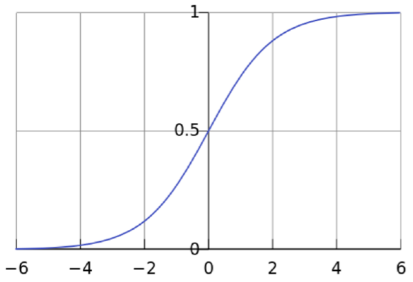
\includegraphics[scale=0.4]{img/sigmoid}
\end{figure}

\subsection{Hyperbolic Tangent function}
\label{ssect:hyperbolic-tangent-function}
\begin{align*}
\sigma(x) = \tanh(x) &= \frac{e^x - e^{-x}}{e^x + e^{-x}} \\
\frac{\delta \sigma(x)}{\sigma(x)} = 1 - \tanh^2(x) &= 1 - \frac{(e^x - e^{-x})^2}{(e^x + e^{-x})^2}
\end{align*}
\begin{figure}[h]
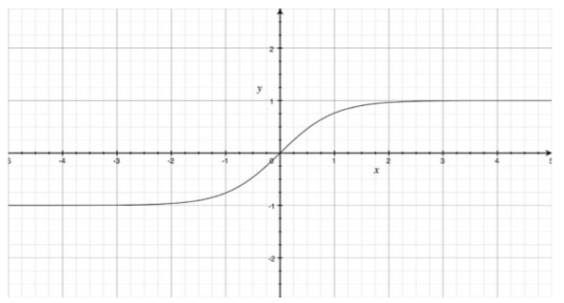
\includegraphics[scale=0.6]{img/tanh}
\end{figure}
If the input has a mean of 0 then so will the output

\subsection{Softmax Function}
\label{ssect:softmax-function}
\begin{align*}
\varphi(x_j) &= \frac{e^{x_j}}{\sum_k e^{x_k}} \\
\frac{\delta \varphi(x_j)}{\varphi(x_j)} = \varphi(x_j) - \varphi(x_j)^2 &= \varphi(x_j)(1 - \varphi(x_j))
\end{align*}
Outputs an a posteriori probability $p(c | x)$ and is good for classification tasks.

\subsection{Rectified Linear Unit}
\label{ssect:softmax-function}
\begin{align*}
\varphi(x) &= max(0,x) \\
\varphi^{'} &= \begin{cases}
1 \: if x > 0\\
0 \: if x \leq 0
\end{cases}
\end{align*}
Can result in sparse networks

\section{Fehlerfunktionen}

\begin{itemize}
\item $E_{MSE}(w) = \frac{1}{2} \sum\limits_{x \in X} \sum\limits_k (t^x_k - o^x_k)^2$
\item Mean-Squared-Error = $\frac{1}{N} * SSE$
\item $E_{CE}(w) = - \sum\limits_{x \in X} \sum\limits_k [t^x_k * log(o^x_k) + (1-t^x_k)*log(1-o^x_k)]$
\end{itemize}

\section{Perzeptron Lernalgorithmus}

$w_{i}^{t+1} = w_i^t + \eta (t_x - o_x) x_i$

\section{Backpropagation}

$w = w - \eta \nabla_w E(x,w)$ mit $\nabla_w E = \frac{\partial E}{\partial o} \frac{\partial o}{\partial \sigma} \frac{\partial \sigma}{\partial w}$

\section{Hopfield}
\begin{align*}
x_j &= \sum_{i; i \neq j} u_i T_{ij} \\
u_i &= g(x_j) = \begin{cases}
1 \: if x \geq 0\\
-1 \: otherwise
\end{cases} \\
E &= - \frac{1}{2} \sum_j \sum_{i;i \neq j} u_i u_j T_{ij} \\
C & \approx 0.15N \\
\frac{N}{4 ln N} < C & < \frac{N}{2 ln N}
\end{align*}
The energy function assigns a numerical value to each possible state of the system (\textbf{Lyapunov Function}.

\section{Boltzmann-Maschinen}
\begin{align*}
z_i &= b_i + \sum_j s_j w_{ij}\\
p(s_i = 1) &= \frac{1}{1 + e^{-z_i}} \\
E &= - \sum_{i < j} w_{ij} s_i s_j - \sum_i b_i s_i \\
p(v) &= \frac{e^{-E(v)}}{\sum_u e^{-E(u)}}
\end{align*}
$b_i$: bias\\
$s_j$: state\\
$w_{ij}$: weight between state j and i\\
\textbf{Simulated Annealing}:
\[
p(s_i = 1) = \frac{1}{1 + e^{-\frac{z_i}{T}}}
\]
\section{Restricted-Boltzmann-Maschinen}
\begin{align*}
E(V, H) &= - \sum_{i=1}^m \sum_{j=1}^F W_{ij} h_j v_i - \sum_{i=1}^m v_i a_i - \sum_{j=1}^F h_j b_j \\
p(h_j = 1 | V) &= \sigma(b_j + \sum_{j=1}^m W_{ij}v_i \\
p(v_i = 1 | H) &= \sigma(a_j + \sum_{j=1}^F W_{ij}h_j \\
\sigma &= \frac{1}{1+e^{-x}}
\end{align*}

\section{Reinforcement Learning}
Bellmanngleichung:
\[
Q^{\pi}(s, a) = \mathbb{E}[r_{t + 1} + \gamma r_{t + 2} + \gamma^2 r_{t + 2} + \gamma^3 r_{t + 3} + ... | s, a]
\]
Recursively:
\[
Q^{\pi}(s, a) = \mathbb{E}_{s^{'}}[r_{t + 1} + \gamma Q^{\pi}(s^{'}, a^{'})| s, a]
\]
Optimal value function:
\[
Q^{*}(s, a) = \mathbb{E}_{s^{'}}[r_{t + 1} + \gamma Q^{\pi}(s^{'}, a^{'})| s, a]
\]
Value iteration solve the Ballman Equation:
\[
Q_{i + 1}(s, a) = \mathbb{E}_{s^{'}}[r_{t + 1} + \gamma Q_i(s^{'}, a^{'})| s, a]
\]
\\[1cm]
Objective function by \textit{mean-squared error} in Q-values:
\[
L(w) = \mathbb{E}[(r + \gamma max_{a^{'}}Q(s^{'}, a^{'}, w^{'} - Q(s, a, w))^2]
\]
Q-learning gradient:
\[
\frac{\delta L(w)}{\delta w} = \mathbb{E}[(r + \gamma max_{a^{'}}Q(s^{'}, a^{'}, w^{'} - Q(s, a, w)) \frac{\delta Q(s, a, w)}{\delta w}]
\]
General TD-learning update rule:
\[
Q(s_t, a_t) += learning_rate \cdot (td_target - Q(s_t, a_t))
\]
TD Target for SARSA:
\[
R_{t + 1} + discount_factor \cdot Q(s_{t + 1}, a_{t + 1})
\]
TD Target for Q-Learning:
\[
R_{t + 1} + discount_factor \cdot maxQ(s_{t + 1}, a_{t + 1})
\]
SARSA
\[
Q(s_t, a_t) += \alpha [r_t + \gamma Q(s_{t+1}, a_{t+1}) - Q(s_t, a_t)]
\]

\section{Generalisierung}

$<\epsilon_{†est}> = <\epsilon_{train}> + 2 \cdot \sigma^2 \frac{p}{n}$ mit Varianz $\sigma$, Parameteranzahl $p$ und Anzahl an Trainingsbeispielen $n$


\section{Normalisierung}

\begin{itemize}
\item Max-Min (Rescaling): $x' = \frac{x - min(x)}{max(x) - min(x)}$
\item Standardisierung: $x' = \frac{x - \bar{x}}{\sigma}$
\item Skalierung auf Einheitslänge: $x' = \frac{x}{||x||}$
\item lückenhafte Daten: Null filling - Smoothing
\end{itemize}

\section{Regularisierung}

\begin{itemize}
\item L1 Norm: $||w||_{L1} = \sum\limits_j |w_j|$
\item L2 Norm: $||w||_{L2} = \sum\limits_j w^2_j$
\item KL-Divergenz:
\[
KL(p || \widehat{p}_j) = p \log(\frac{p}{\widehat{p}_j}) + (1 - p) \log(\frac{1 - p}{1 - \widehat{p}_j})
\]
\item Cross-Entropy: $E_{CE}(w) = - \sum\limits_{x \in X} \sum\limits_k [t^x_k * log(o^x_k) + (1-t^x_k)*log(1-o^x_k)]$
\item Edit-Distance: 
\item Dropout: 
\item Meiosis: Idea: adding of hidden unis depends on the ''uncertainty'' of the network. The mean and varianz is learned.
\[
w_{ij}^{*} = \mu(w_{ij}) + \sigma(w_{ij}) \phi(0, 1)
\]
Start with one hidden unit and split unit if
\[
\frac{\sum_i \sigma_{ij}}{\sum_i \mu_{ij}} > 1.0 \: and \: \frac{\sum_k \sigma_{ik}}{\sum_k \mu_{ik}} > 1.0
\]
\end{itemize}

\section{Adaptive Lernratenanpassung}

\begin{itemize}
\item AdaGrad: $w_t = w_{t-1} - \frac{\eta}{\sqrt{G_t+\epsilon}} L(x,w_{t-1})$ mit der Diagonalmatrix $G_t$, die die Beträge des Gradienten enthält und $\epsilon$: Smoothingterm, um Division durch 0 zu verhindern
\item $w_t = w_{t-1} - \frac{RMS[\Delta w]_{t-1}}{RMS[g]_t}g_t$, wobei $RMS[\Delta w]_t$ der \glqq root mean squared error\grqq\ $\sqrt{E[\Delta w^2]_t + \epsilon}$ ist.
\item RMSProp: $w_t = w_{t-1} - \frac{\eta}{\sqrt{E[g^2]_t + \epsilon}} g_t$
\end{itemize}

\section{Updates für Backprop}

\begin{itemize}
\item Momentum-Term: $\Delta w_{ij}(t) = - \eta \frac{\partial E}{\partial w_{ij}(t)} + \alpha * \Delta w_{ij}(t-1)$
\item QuickProp: \[
\Delta w(t) = \frac{s(t)}{s(t - 1) - s(t)} \cdot \Delta w(t-1)
\]
\item WeightElimination: \[
E = MSE + \lambda \sum_{i,j} \frac{w_{i,j}^2}{1 + w_{i,j}^2}
\]
\end{itemize}

\section{Autoencoders}
Durchschnittliche Aktivierung von Sparse Autoencoder: 
\[
\widehat{p_j} = \frac{1}{|N|} \sum_{x \in X} w_j x
\]
force this average activation to be p $\approx$ 0.2 by adding the Kullback–Leibler divergence $KL(p || \widehat{p_j})$ to the error function
\section{Shared Weights bei TDNNs}
\begin{itemize}
	\item[1.]$w_j^{t_1} = w_j^{t_2} \Rightarrow \Delta w_j^{t_1} = \Delta w_j^{t_2}$
	\item[2.]Berechne $\frac{\partial E}{\partial w_j^{t_1}}$ und $\frac{\partial E}{\partial w_j^{t_2}}$
	\item[3.] $\Delta w_j^{t_1} = \Delta w_j^{t_2} = -\eta \left(\frac{\partial E}{\partial w_j^{t_1}} + \frac{\partial E}{\partial w_j^{t_2}}\right)$
\end{itemize}


\section{Gewichtsupdate mit $cos$}

\begin{figure}[h]
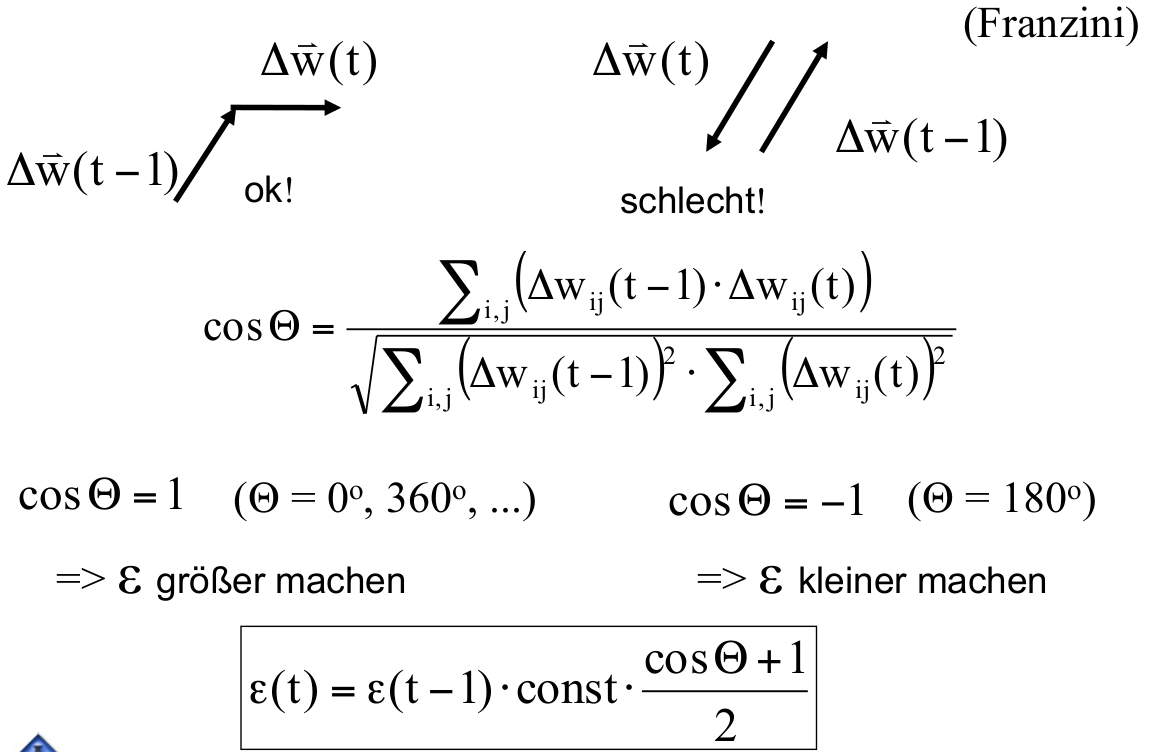
\includegraphics[scale=0.3]{img/dynamic-learning-rate}
\end{figure}

\section{LVQ}

\subsection{LVQ1}
\label{sssect:vq-lvq1}
$c = argmin_i\{||x - m_i||\}$: Index des prototype vectors\\
Learning rules:
\begin{itemize}
	\item $m_c(t + 1) = m_c(t) + \alpha(t)[x(t) - m_c(t)]$: $x$ und $m_c$ selbe Klasse
	\item $m_c(t + 1) = m_c(t) - \alpha(t)[x(t) - m_c(t)]$: $x$ und $m_c$ unterschiedliche Klasse
	\item $m_c(t + 1) = m_i(t)$: für $i \neq c$
\end{itemize}

\subsection{LVQ2}
\label{sssect:vq-lvq2}
Die Klassifizierung ist die selbe wie bei LVQ1. Das updaten ist anders:
\begin{itemize}
	\item $m_i$ und $m_j$ sind die nähsten Nachbarn von $x$ und werden simulaten geupdated.
	\item $x$ muss in ein ''window'' um $m_i$ und $m_j$ fallen.
	\item $d_i$ und $d_j$ sind die Distanzen (z.B. euklidien) zwischen $x$ und $m_i$ und $m_j$
	\item $min \left(\frac{d_i}{d_j}, \frac{d_j}{d_i}\right) > s$ where $s = \frac{1 - w}{1 + w}$ (recommended window: 0.2 to 0.3)
\end{itemize}


Ergänzungen:
$m_i$ ist der Gewinner (falsche klasse)
$m_j$ zweiter gewinner, richtige klasse -> dann updaten
$\alpha$ die Lernrate wird kleiner und kleiner

\end{document}